\epigraph{\textit{Information flow is what the Internet is about. Information sharing is power. If you don't share your ideas, smart people can't do anything about them, and you'll remain anonymous and powerless.}}{-- \textup{Vint Cerf}}

We have seen thus far the two main export formats supported by Wikidata, namely, RDF and JSON. However, none of them are suitable for analytical queries. In this chapter, we will explore the possibility of exporting Wikidata in a columnar format, as we have mentioned in the previous chapter, DuckDB is the perfect candidate for this task. Putting this all together, we will create a Rust-based solution for exporting Wikidata to DuckDB.

\section{The issue with JSON and other text-based formats}
\label{section:issue}

JSON is a text-based format, and as such, the data that is stored inside a JSON file is not compressed in any way. This means that the size of the file is directly proportional to the size of the data. This is not a problem for small datasets, but it becomes an issue when we are dealing with larger information repositories. As we have seen in the introductory chapter a Wikidata JSON dump is around \texttt{1.5 TB} in size when uncompressed, see \ref{chapter:intro} for a more detailed explanation. The problem here is that we cannot store such a large file on a single machine. Even if we could, it would take quite a time to load the whole file into memory. As a result, a binary format is required to store the information. This is where DuckDB comes into play. Even if we are also required to load the database into memory; recall, DuckDB is an in-process or embedded database, and the size of the repository is much smaller than the one of the JSON file; orders of magnitude smaller to say the least. This is because DuckDB is a columnar database, and as such, it can compress the data much more efficiently than a text-based format. This is the main reason why we want to export Wikidata to DuckDB.

It is also worth noting that Wikidata JSON dumps are structured in such a way that per each line of the file, one object is stored. This means that we can parse the file line by line, which is something cool. However, it comes with the downside that every line of the dump will contain boilerplate information referring to the schema of the JSON objects. What I mean by this is that we will potentially have hundreds of millions of lines all of them with the same boilerplate code. Instead of having a header with the schema of the JSON object, it will be repeated at each of the lines of the document. This is one of the reasons why JSON files are not efficient memory-wise. For sharing information, JSON is great, but for storing it, it is not.

\section{wd2duckdb}

Now that we have a clear understanding of the scope of the project, we can start working on the design of the tool in charge of transforming the Wikidata JSON dumps into a DuckDB file. For us to do so, some restrictions are going to be considered. First, we are interested in storing only one of the translations for each Wikidata entity; that is, we are going to store only one of the labels, descriptions, and aliases for each item. The language of choice can be modified\footnote{\url{https://github.com/angelip2303/wd2duckdb/blob/master/wikidata-rs/src/lib.rs\#L20}}. Second, we are going to store only the statements that are not deprecated. Apart from that, the rest of the information is going to be preserved.

\label{section:wd2duckdb_design}
\subsection{Design}

The tool is going to be divided into two main parts. The first part is going to be in charge of parsing the Wikidata JSON dump and extracting the information that we are interested in. The second part is going to be in charge of storing the information in a DuckDB database. The idea is to allow backends to be interchangeable; that is, several implementations for other drivers should be implemented without actually changing the existing code. However, for the sake of simplicity, we are going to focus on DuckDB for the time being.

\begin{figure}[ht]
    \centering
    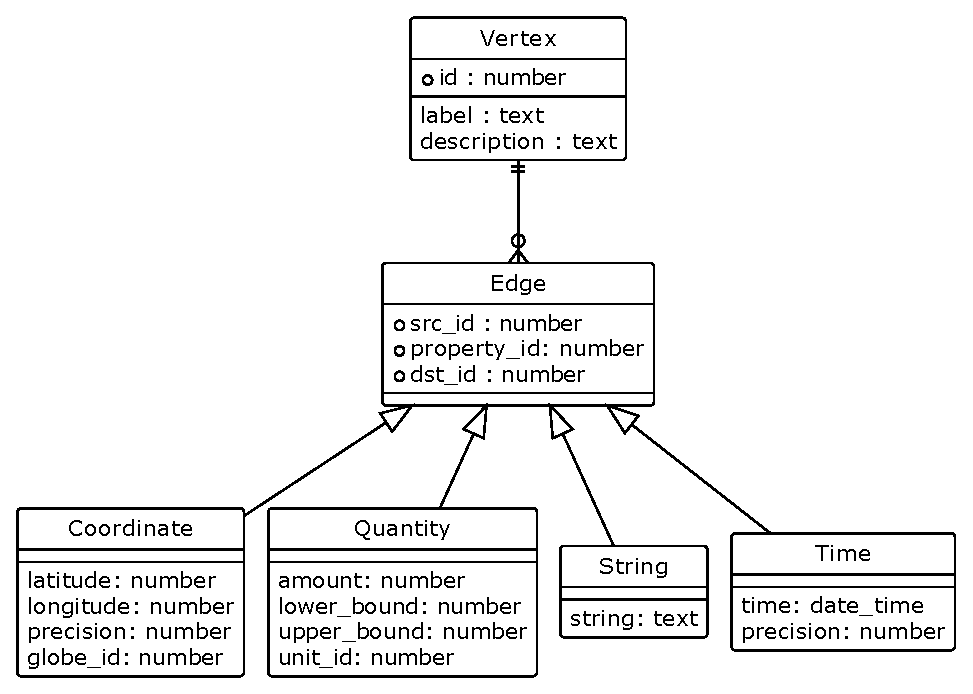
\includegraphics[width=.8\linewidth]{img/10-1_wd2duckdb.eps}
    \caption{Entity-relationship diagram of \texttt{wd2duckdb}'s resulting Database}
\end{figure}%

\subsubsection{Parsing the JSON dump}

The first part of the tool is going to be in charge of parsing the Wikidata JSON dump and extracting the information that we are interested in. The idea is to parse the file line by line, and for each line, we are going to extract the information that we are interested in. Having that said, the information that we are going to extract is the following:

\begin{itemize}
    \itemsep0.5em
    \item \textbf{Wikidata IDs}: As we had seen in section \ref{section:wikibase_graphs}, Wikidata IDs consist of a type prefix \texttt{Q}, \texttt{P} or \texttt{L}, for identifying Entities, Properties or Lexemes, followed by a sequence of numbers. There exist other two types of IDs, namely, \texttt{F} and \texttt{S}, for identifying Forms and Senses, respectively. A more detailed discussion on this topic will be presented later on. For the time being, we are going to focus on the first three types of IDs. The idea is to store the IDs in a separate table, and then, for each line of the JSON dump, we are going to store the ID of the entity that is being parsed. This is going to be useful for the second part of the tool, where we are going to store the statements of the entities.
    \item \textbf{Labels}: We are going to store the labels of the entities in the same table where we store the IDs.
    \item \textbf{Descriptions}: We are going to store the descriptions of the entities in the same table where we store the IDs.
    \item \textbf{Statements}: We are going to store the statements of the entities in a separate table so that we can build the graph later on. The idea is to store the ID of the source entity, the ID of the property and the ID of the destination entity. In this manner, we will end up with two main tables: one for storing the entities, or vertices, and another one for storing the statements, or edges. Several other tables are going to be created for storing data relative to the information that comes with the statements, such as qualifiers, references, ranks, etc. However, for the time being, we are going to focus on the main tables.
\end{itemize}

\subsubsection{Optimizations}

The Wikidata JSON dump is a huge file. As we have seen in section \ref{section:issue}, the file is around \texttt{1.5 TB} in size. This means that we need to put an extra effort into optimizing the tool. For that, we are going to use a combination of different techniques, such as compression, and fine-tuning the chosen data types.

\paragraph{Compression}





\subsection{Implementation of the \texttt{wd2duckdb} tool}

The information that we have gleaned from the JSON dump will be kept in a DuckDB database by the tool's second component. The idea here is to create a Rust-based solution that can be used as a library or as a command-line tool. This CLI will act as a wrapper for the library and be responsible for calling it as well as handling command-line inputs such as the source JSON and the target file. Through \texttt{crates.io}\footnote{\url{https://crates.io/crates/wikidata-rs}}, we aim to make the library available to other Rust-based projects. This is, we are looking to decouple the library from the command-line tool for other backends to be implemented on top of the same traits.

\subsection{Quality assurance}

In the following subsections, we are going to discuss the different quality assurance mechanisms that we are going to use for the development of the tool. The idea is to ensure that the tool is robust and that it can be used in production environments. For that, we are going to use a combination of different techniques, such as version control, documentation, testing, continuous integration and continuous deployment. Note that the tool is going to be open-source, which means that the community will be able to contribute to the project. This is going to be beneficial for the project as it will allow us to have a more robust tool. Lastly, note that we are going to use this same methodology for the development of the other tools that we are going to develop in this thesis.

\subsubsection{Version control}

Recall that we are building an open-source solution. Hence, we are going to use Git as our version control system. The idea is to use GitHub as our remote repository. This will allow us to have a public repository where the community can contribute to the project. Moreover, we are going to use Git tags for the versioning, letting us have a clear understanding of the different versions of the tool. For instance, we are using the \texttt{v0.0.1} tag for the first version. Subsequent versions will be annotated with a \texttt{v0.0.x} tag. What's more, for the sake of simplicity, we are going to use \textit{stable mainline} as our branching strategy for the development of the tool. This means that we are going to have a \texttt{main} branch where the latest stable version is going to be stored. The idea is to have a \texttt{dev} branch where the heavy duty in the development is going to take place. Once we have a stable version, we will merge it into the \texttt{main} branch. Note that this is a simple branching strategy that will work just fine for the development of this project as I am the only developer. However, for larger projects, a more complex branching strategy should be used.

\subsubsection{Documentation}

Having that said, writing good documentation is essential for the development of a robust tool. For that, we are going to use Rust's documentation tool, namely, \texttt{rustdoc}. The idea is to document the different functions and methods of the tool so that the community can have a clear understanding of the tool's API. Moreover, we are going to use \texttt{rustdoc}'s \texttt{doc-tests} feature for writing tests in the documentation. Putting this all together, the whole documentation will be deployed to \texttt{docs-rs}\footnote{\url{https://docs.rs/wikidata-rs/0.0.1/wikidata_rs/}}.

\subsubsection{Testing}

The idea is to have a robust tool that can be used in production environments. For that, we are going to use Rust's testing framework, namely, \texttt{cargo test}. The idea is to write unit tests for the different functions and methods of the tool.

\subsubsection{Continuous integration and continuous deployment}

The result of combining the previous techniques results in a robust tool that can be used in production environments. However, we are going to take it one step further by using continuous integration and continuous deployment. The idea is to make use of GitHub Actions. The idea is to have an Action that will run the tests of the tool every time a new commit is pushed to the repository's \texttt{main} branch. This will allow us to have a clear understanding of the state of the tool. Moreover, we are going to have another GitHub Action that will be in charge of deploying the tool to the \texttt{crates.io}\footnote{\url{https://crates.io}} platform.